\documentclass[12pt]{article}
\usepackage{amsfonts, epsfig}
\usepackage[authoryear]{natbib}
\usepackage{graphicx}
\usepackage{fancyhdr}
\usepackage{amsmath}
\usepackage{xcolor}
\pagestyle{fancy}
\lfoot{\texttt{coms10013.github.io}}
\lhead{Analysis - 5. Approximating functions and Taylor expansion}
\rhead{\thepage}
\cfoot{}
\begin{document}

In this lecture, we're going to take a glimpse into approximating functions. Sometimes functions are very complicated and difficult to compute or understand. By using approximations of the function, we lose information about our function; on the other hand, the function becomes significantly more malleable and we gain understanding about how it behaves. 

The goal of this lecture is to look at the Taylor series expansion of a function: this gives a way to write any differentiable function $f(x)$ as an infinite sum of polynomial terms (i.e. $x, x^2, x^3,\dots$. 

\section*{Linear approximation of a function}
Let $f(x)$ be a differentiable function. Then the \textbf{linear approximation} of $f$ at $x = a$ is 
\begin{equation}
    L(x) = f(a) + f'(a) (x-a)\,.
\end{equation}

This gives a way to understand $f$ as a linear expression at the coordinates $(a, f(a))$. Geometrically, this is akin to taking the tangent of $f$ at $a$, and saying that, locally, $f$ looks like this tangent line. 

Let's look at an example: suppose we'd like to approximate the (admittedly not particularly complicated) function $f(x) = x^2$ at the point $a=3$. Note that $f$ is differentiable. Using the above formula, we find that the approximation is 
\begin{align*}
    L(x) &= a^2 + 2a(x-a)\\
    & = 9 + 6(x-3)\\
    & = 6x - 9\,.
\end{align*}
From this, we conclude that if we were to look at $f(x)$ at $x=a$, and pretend that it were a line (i.e. take its linear approximation), then the line would have the equation $y = 6x-9$.

\section*{Finding roots: Newton's method}
Already this coarse linear approximation of a function can be very useful. Often, when understanding a function $f(x)$, we want to ask questions such as `for what values of $x$ is $f(x) =0$". In other words, can we find a root of $f$. 

Newton's method is a way of finding roots using the linear approximation of $f$. It is an iterative method, and typically fairly powerful. In its favour is also that the procedure itself is very simple. We begin with an initial value $x_0$. Then 
\begin{equation}
    x_{n+1} = x_n - \frac{f(x_n)}{f'(x_n)}\,.
\end{equation}

Let's try an example: suppose we'd like to find roots of the function $f(x) = x^2 - 1$. Clearly we know that $x=1$ is a root (since $f(1) = 0$), but for the purposes of this example, we shall pretend that we do not know this. Let's start with an initial value $x_0=13$, and see what happens:\\
\begin{itemize}
    \item $x_1 = 13 - \frac{13^2 - 1}{2\times13} = 6.528\dots$
    \item $x_2 = 6.528 - \frac{6.528^2 -1 }{2\times 6.528} = 3.345\dots$
\end{itemize}
We can continue in this fashion to find that $x_3 = 1.822...$, and eventually $x_7 = 1.0000000053931304$, and (at least with the approximation of floating numbers in Python), $x_8 = 1.0$. So, very quickly (and with very little thought), we found a root of $f$.

Newton's method requires $f$ to be differentiable, and also that $f'(x_i)\neq 0$. 

Geometrically, Newton's method works by using the linear approximation function as a tangent to the curve at $f(x_i)$; the subsequent value $x_{i+1}$ is the abscissa\footnote{Fancy word for $x$-value; the \emph{ordinate} is the fancy word for the $y$ value of a coordinate.} for where the tangent line intercepts the $x$-axis. 

More mathematically, the linear approximation of $f$ at $x_0$ is given by
\[
L(x_1) = f(x_0) + f'(x_0)(x_1 - x_0)\,;
\]
because we want a root of $f$, we aim for the left-hand side to be zero. Rearranging gives us the value of $x_1$ that we need, namely
\[
x_1 = x_0 - \frac{f(x_0)}{f'(x_0)}\,,
\]
and we iterate the process to find subsequent values of $x_i$.

Typically we'll stop this process once $x_i$ and $x_{i+1}$ are sufficiently close, according to some threshold that we choose. 



\section*{The Taylor expansion}
Suppose we have temporarily forgotten\footnote{An admittedly unlikely situation.} that one of our favourite numbers $e$ is actually $2.71828\dots$, but that we find ourselves needing to calculate $\exp(7)$. Can we do this? 

Surprisingly, the answer is yes! That's assuming that we're interpreting the exponential as a bona fide function $\exp:\mathbb{R}\to \mathbb{R}$ that we can differentiate. In fact, we'll need to use a definition of $\exp$ that is $\frac{d}{dx}\exp(x) = \exp(x)$. To do this, we'll use the \emph{Taylor series expansion}.

More generally, the Taylor series allows us to take a function that is hard to calculate (but whose derivate at certain points exists and is computable), and to approximate it. Importantly, the approximation is to a polynomial function: the Taylor series lets us write any\footnote{A slight exaggeration: any function that is differentiable at some point $a$.} function $f(x)$ as an infinite series of the form 
\[
f(x) = \sum_{i=0}^{\infty}a_i x^i 
\]
where the $a_i$ are some values that we determine (using higher order derivatives). Typically, we'll approximate $f$ by truncating the series to make it a sum of a finite number (say $T$) terms:
\[
f(x) \approx \sum_{i=1}^T a_i x^i
\]
and the bigger we take $T$, the more accurate the approximation. 

This leaves the burning question: how do we calculate the $a_i$ terms? 

\subsection*{How to calculate the Taylor series}
Suppose that we'd like to approximate a function $f$ at the point $x=a$ by a polynomial of degree $M$, and that we know $f(a), f'(a), ..., f^{(M)}(a)$ (i.e. the order $M$ derivatives at $a$; we require also that these derivatives exist).

In other words, we'd like $f(x)$ to look like:
\[
g(x) = c_0 + c_1(x-a) + c_2 (x-a)^2 + \dots + c_M(x-a)^M\,.
\]

Now some observations:
\begin{itemize}
\item  $g(a) = c_0$ (this is why we wrote $g$ a little unintuitively as a sum of $(x-a)$ powers). 
\item Differentiating both sides gives $g'(x) = c_1 + 2c_2(x-a)+\dots$, so that $g'(a) = c_1$. 
\item Finding the second order derivative, we get $g''(x) = 2c_2+\dots$, where the $\dots$ involves terms that are multiples of $(x-a)$ so that they disappear when we evaluate $g''(a)$. Thus, $g''(a) = 2c_2$.
\item Finding the third order derivative, we get $g'''(x) =g^{(3)}(x)= 3\times 2c_3+\dots$, where the $\dots$ involves terms that are multiples of $(x-a)$ which again disappear when $x=a$. Thus, $g''(a) = 3!c_3 = 6c_3$.
\item Continuing in this manner, we get that $g^{(n)}(a) = n!c_n$.
\end{itemize}

Let's now recall our initial goal: to approximate $f(x)$ by a polynomial $g(x)$:
\[
f(x) \approx g(x)\,.
\]
We'll differentiate both sides and evaluate the derivative at $x=a$; we then match up the coefficients. Let's evaluate the $n$th order derivative on both sides: the $n$th order derivative of $f$ at $a$ is simply $f^{(n)}(a)$; when we evaluate the $n$th order derivative of $g$ at $a$, we'll find that the only non-zero term is the term that comes from differentiating $c_n(x-a)^n$. In other words, 
\[
f^{(n)}(a) =  n!c_n\,.
\]

Hence our Taylor series expansion of $f(x)$ at the point $x=a$ is 
\begin{equation}\label{eq:taylor}
\sum_{i=0}^M \frac{(x-a)^i}{i!}f^{(i)}(a)\,.
\end{equation}
Recall that $0! = 1$.

\subsection*{Example}
Let's use the Taylor series to understand the exponential function $\exp(x)$.  We'd like to approximate at $x=0$ (so taking $a=0$ in the definition).

Firstly, let's evaluate the higher order derivatives: we know (for instance by the definition of the $\exp(\cdot)$ function that
\[
\frac{d}{dx}\exp(x) = \exp(x)\,.
\]
This means that 
\[
\frac{d^{n}}{dx^n}\exp(x) = \exp(x)\,.
\]
(One way that you could convince yourself of this is by using \emph{proof by induction} that you learnt about in Maths A.)
Putting this into \eqref{eq:taylor}, we get that an order $M$ approximation of $\exp(x)$ is
\[
\exp(x)\approx \sum_{i=0}^M \frac{x^i}{i!}\exp(0)
= \sum_{i=0}^M \frac{x^i}{i!}\,.
\]

So if we wanted to calculate $\exp(7)$ using a 20th order approximation, we'd set $M=20$ and calculate the first 21 (because we start counting at $i=0$ terms of this expression:
\begin{align*}
\exp(7) \approx 1+ &7 + 24.5+ 57.167 + 100.04 + \\
&+ 140.06+163.40+163.40+142.98+111.20+77.84+\\
&  +49.54 +28.90 + 15.56 + 7.78 + 3.63 + 1.59  + 0.65 + 0.25 + 0.09.
\end{align*}
Hopefully you'll notice that these numbers initially grow, and then rapidly shrink again. This is typical behaviour: eventually the contribution from the later terms will become less important. 

Summing up these terms we find that $\exp(7) \approx 1096.58$. When we compare this to the actual value $e^7 = 1096.63$, we can  persuade ourselves that these numbers do indeed match very closely. 


\subsection*{Considerations}
We haven't yet said very much about when then Taylor expansion works: for example, $f(x)$ might have funny
behaviour. For example if $f(x)=x+1/x$ then the Taylor expansion
around $x=0$ wouldn't work. Indeed $f(x)$ goes to infinity as $x$
gets closer to zero. In that case, there is a more general version of
the Taylor expansion that works, the \textbf{Laurent series}; we don't
look at that here. 

We have also ignored the issue of convergence; does
the error in not doing the sum all the way to infinity get smaller as
we take more terms. It seems likely that this is the case since the
$1/n!$ term gets very large, in fact, this is not generally true,
there are functions for which the series does not work, but, again, we
are going to ignore that here and think about the large class of
well-behaved functions whose Taylor expansions are well-behaved.

More generally, there is an interesting issue here; for the class of these
well-behaved functions, called \textbf{analytic functions}, the Taylor
expansion seems to say that there are two ways to write down the
function, for a function which is analytic around $t=0$, in the first
description $f(t)$ gives a value for $f$ at each value $t$, in the
second, describes the function in terms of the derivatives, $f(0$,
$f'(0)$, $f''(0)$ and so on, with the Taylor expansion translating
from the second description back to the first. 

\subsection*{Another example}
Let's look at another example,
\begin{equation}
  f(t)=\cos{t}
\end{equation}
around $t=0$. Now $f'(t)=-\sin{t}$ and $f''(t)=-\cos{t}$ and
$f'''(t)=\sin{t}$ and $f^{(4)}(t)=\cos{t}$ and after that the cycle
repeats. Using $\sin{0}=0$ and $\cos{0}=1$ this tells us that
\begin{equation}
  \cos{t}=1-\frac{1}{2}t^2+\frac{1}{24}t^4-\frac{1}{720}t^6+\ldots
\end{equation}
We can see how well this works in Figure~1.
\begin{figure}[h!]
  \begin{center}
    % GNUPLOT: LaTeX picture with Postscript
\begingroup
  \makeatletter
  \providecommand\color[2][]{%
    \GenericError{(gnuplot) \space\space\space\@spaces}{%
      Package color not loaded in conjunction with
      terminal option `colourtext'%
    }{See the gnuplot documentation for explanation.%
    }{Either use 'blacktext' in gnuplot or load the package
      color.sty in LaTeX.}%
    \renewcommand\color[2][]{}%
  }%
  \providecommand\includegraphics[2][]{%
    \GenericError{(gnuplot) \space\space\space\@spaces}{%
      Package graphicx or graphics not loaded%
    }{See the gnuplot documentation for explanation.%
    }{The gnuplot epslatex terminal needs graphicx.sty or graphics.sty.}%
    \renewcommand\includegraphics[2][]{}%
  }%
  \providecommand\rotatebox[2]{#2}%
  \@ifundefined{ifGPcolor}{%
    \newif\ifGPcolor
    \GPcolortrue
  }{}%
  \@ifundefined{ifGPblacktext}{%
    \newif\ifGPblacktext
    \GPblacktexttrue
  }{}%
  % define a \g@addto@macro without @ in the name:
  \let\gplgaddtomacro\g@addto@macro
  % define empty templates for all commands taking text:
  \gdef\gplbacktext{}%
  \gdef\gplfronttext{}%
  \makeatother
  \ifGPblacktext
    % no textcolor at all
    \def\colorrgb#1{}%
    \def\colorgray#1{}%
  \else
    % gray or color?
    \ifGPcolor
      \def\colorrgb#1{\color[rgb]{#1}}%
      \def\colorgray#1{\color[gray]{#1}}%
      \expandafter\def\csname LTw\endcsname{\color{white}}%
      \expandafter\def\csname LTb\endcsname{\color{black}}%
      \expandafter\def\csname LTa\endcsname{\color{black}}%
      \expandafter\def\csname LT0\endcsname{\color[rgb]{1,0,0}}%
      \expandafter\def\csname LT1\endcsname{\color[rgb]{0,1,0}}%
      \expandafter\def\csname LT2\endcsname{\color[rgb]{0,0,1}}%
      \expandafter\def\csname LT3\endcsname{\color[rgb]{1,0,1}}%
      \expandafter\def\csname LT4\endcsname{\color[rgb]{0,1,1}}%
      \expandafter\def\csname LT5\endcsname{\color[rgb]{1,1,0}}%
      \expandafter\def\csname LT6\endcsname{\color[rgb]{0,0,0}}%
      \expandafter\def\csname LT7\endcsname{\color[rgb]{1,0.3,0}}%
      \expandafter\def\csname LT8\endcsname{\color[rgb]{0.5,0.5,0.5}}%
    \else
      % gray
      \def\colorrgb#1{\color{black}}%
      \def\colorgray#1{\color[gray]{#1}}%
      \expandafter\def\csname LTw\endcsname{\color{white}}%
      \expandafter\def\csname LTb\endcsname{\color{black}}%
      \expandafter\def\csname LTa\endcsname{\color{black}}%
      \expandafter\def\csname LT0\endcsname{\color{black}}%
      \expandafter\def\csname LT1\endcsname{\color{black}}%
      \expandafter\def\csname LT2\endcsname{\color{black}}%
      \expandafter\def\csname LT3\endcsname{\color{black}}%
      \expandafter\def\csname LT4\endcsname{\color{black}}%
      \expandafter\def\csname LT5\endcsname{\color{black}}%
      \expandafter\def\csname LT6\endcsname{\color{black}}%
      \expandafter\def\csname LT7\endcsname{\color{black}}%
      \expandafter\def\csname LT8\endcsname{\color{black}}%
    \fi
  \fi
    \setlength{\unitlength}{0.0500bp}%
    \ifx\gptboxheight\undefined%
      \newlength{\gptboxheight}%
      \newlength{\gptboxwidth}%
      \newsavebox{\gptboxtext}%
    \fi%
    \setlength{\fboxrule}{0.5pt}%
    \setlength{\fboxsep}{1pt}%
    \definecolor{tbcol}{rgb}{1,1,1}%
\begin{picture}(5040.00,3440.00)%
    \gplgaddtomacro\gplbacktext{%
      \csname LTb\endcsname%%
      \put(616,769){\makebox(0,0)[r]{\strut{}$-1$}}%
      \csname LTb\endcsname%%
      \put(616,1351){\makebox(0,0)[r]{\strut{}$-0.5$}}%
      \csname LTb\endcsname%%
      \put(616,1934){\makebox(0,0)[r]{\strut{}$0$}}%
      \csname LTb\endcsname%%
      \put(616,2516){\makebox(0,0)[r]{\strut{}$0.5$}}%
      \csname LTb\endcsname%%
      \put(616,3099){\makebox(0,0)[r]{\strut{}$1$}}%
      \csname LTb\endcsname%%
      \put(789,448){\makebox(0,0){\strut{}$-\pi$}}%
      \csname LTb\endcsname%%
      \put(1747,448){\makebox(0,0){\strut{}$-\pi/2$}}%
      \csname LTb\endcsname%%
      \put(2706,448){\makebox(0,0){\strut{}$0$}}%
      \csname LTb\endcsname%%
      \put(3664,448){\makebox(0,0){\strut{}$\pi/2$}}%
      \csname LTb\endcsname%%
      \put(4622,448){\makebox(0,0){\strut{}$\pi$}}%
    }%
    \gplgaddtomacro\gplfronttext{%
      \csname LTb\endcsname%%
      \put(2705,142){\makebox(0,0){\strut{}$t$}}%
      \csname LTb\endcsname%%
      \put(3818,3032){\makebox(0,0)[r]{\strut{}$\cos{t}$}}%
      \csname LTb\endcsname%%
      \put(3818,2828){\makebox(0,0)[r]{\strut{}two terms}}%
      \csname LTb\endcsname%%
      \put(3818,2624){\makebox(0,0)[r]{\strut{}three terms}}%
      \csname LTb\endcsname%%
      \put(3818,2420){\makebox(0,0)[r]{\strut{}four terms}}%
    }%
    \gplbacktext
    \put(0,0){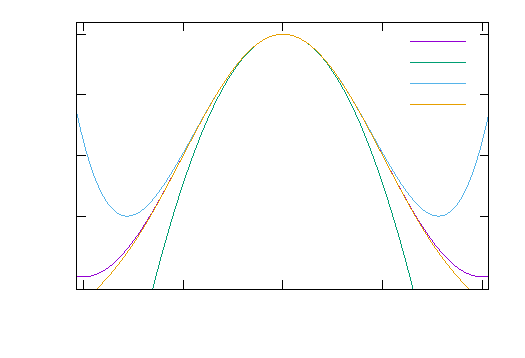
\includegraphics[width={252.00bp},height={172.00bp}]{cos}}%
    \gplfronttext
  \end{picture}%
\endgroup
    \end{center}
  \caption{A comparison of $\cos{t}$ with successive terms of Taylor expansion; we see the approximation getting better and better, at least in the range we are looking at; the labelling of the terms is the number of non-zero terms included.}
\end{figure}

\section*{Summary}
We looked at using the derivative to find a linear approximation of a function. This was a mathematical way to say `take the gradient of the function at the point'.

This mathematical interpretation of taking the gradient via the derivative let us calculate the roots of the function using the very simple but very powerful Newton method: $x_{n+1} = x_n-\frac{f(x_n)}{f'(x_n)}$.

We might want a better approximation to our function than a merely linear one: for this, we use the Taylor expansion. 

The main thing to remember is the Taylor expansion itself:
\begin{equation}
  f(t+\delta t)=f(t)+\sum_{n=1}^\infty \frac{1}{n!}f^{(n)}(t)\delta t^n
\end{equation}
\end{document}

